\vspace{-0.3cm}
\section{Algorithms for Few-Shot Object Detection}

In this section, we start with the preliminaries on the few-shot object detection setting. Then, we talk about our two-stage fine-tuning approach in
Section~\ref{sec:tfa}. Section~\ref{sec:meta} summarizes the previous meta-learning approaches.

% \minisection{Few-shot object detection preliminaries.}
We follow the few-shot object detection settings introduced in~\citet{kang2019few}. There are a set of base
classes $C_b$ that have many instances and a set of novel classes $C_n$ that
have only $K$ (usually less than 10) instances per category.
For an object detection dataset $\mathcal{D}=\{(x, y), x\in\mathcal{X}, y\in\mathcal{Y}\}$, where $x$
is the input image and $y=\{(c_i, \vec{l}_i), i=1, ...,N\}$ denotes the categories $c \in C_b \cup C_n$
and bounding box coordinates $\vec{l}$ of the $N$ object instances in the image $x$.
% $y=\{(c^i, x_1^i, x_2^i, y_1^i, y_2^i), i=1, ...,N\}$
For synthetic few-shot datasets using
COCO, the novel set for training is balanced and each class has the same number of 
annotated objects (\textit{i.e.}, $K$-shot). The recent LVIS dataset has a natural long-tail distribution, which does
not have the manual $K$-shot split. The classes in LVIS are divided into \emph{frequent} classes
(appearing in more than 100 images), \emph{common} classes (10-100 images), and \emph{rare}
classes (less than 10 images). We consider both synthetic and natural datasets in our work and
follow the naming convention of $k$-shot for simplicity. 

The few-shot object detector is evaluated on a test set of both the base classes and
the novel classes. The goal is to optimize the detection accuracy measured by average precision (AP)
of the novel classes as well as the base classes. This setting is different from the $N$-way-$K$-shot setting~\cite{finn2017model,vinyals2016matching,snell2017prototypical}
commonly used in few-shot classification. 

\subsection{Two-stage fine-tuning approach}
\label{sec:tfa}
We describe our two-stage fine-tuning approach (\model) for few-shot object detection in
this section. We adopt the widely used Faster R-CNN~\cite{ren2015faster}, a two-stage object
detector, as our base detection model. As shown in Figure~\ref{fig:tfa_arch}, the feature learning components, referred to as $\mathcal{F}$, of a Faster R-CNN model include the backbone (\textit{e.g.}, ResNet~\cite{he2016deep}, VGG16~\cite{simonyan2014very}), the region proposal network (RPN), as well as a two-layer
fully-connected (FC) sub-network as a proposal-level feature extractor. 
There is also a box predictor composed of a box classifier $\mathcal{C}$ to classify the
object categories and a box regressor $\mathcal{R}$ to predict the bounding box coordinates. 
Intuitively, the backbone features as well as the RPN features
are class-agnostic. Therefore, features learned from the base classes are likely to transfer
to the novel classes without further parameter updates. The key component of our method is to separate the
feature representation learning and the box predictor learning into two stages. 

\minisection{Base model training.} In the first stage, we train the feature extractor 
and the box predictor only on the base classes $C_b$, with the same loss function used in ~\citet{ren2015faster}. The joint loss is, 
\begin{equation}
    \mathcal{L} = \mathcal{L}_{\text{rpn}} + \mathcal{L}_{\text{cls}} + \mathcal{L}_{\text{loc}},
    \label{eq:loss}
\end{equation}
where $\mathcal{L}_\text{rpn}$ is applied
to the output of the RPN to distinguish foreground from backgrounds and refine the
anchors, $\mathcal{L}_\text{cls}$ is a cross-entropy loss for the box classifier $\mathcal{C}$,
and $\mathcal{L}_\text{loc}$ is a smoothed $L_1$ loss for the box regressor $\mathcal{R}$.

\minisection{Few-shot fine-tuning.} In the second stage, we create a small balanced training set 
with $K$ shots per class, containing both base and novel classes.
% We add randomly initialized weights of the novel classes to the trained box predictor
We assign randomly initialized weights to the box prediction networks for the novel classes
and fine-tune only the box classification and
regression networks, namely the last layers of the detection model, while keeping the entire 
feature extractor $\mathcal{F}$ fixed. We use the same loss function
in Equation~\ref{eq:loss} and a smaller learning rate. The learning rate is reduced by 20 from the first stage in all our experiments. 

\begin{figure*}[ht]
    \centering
    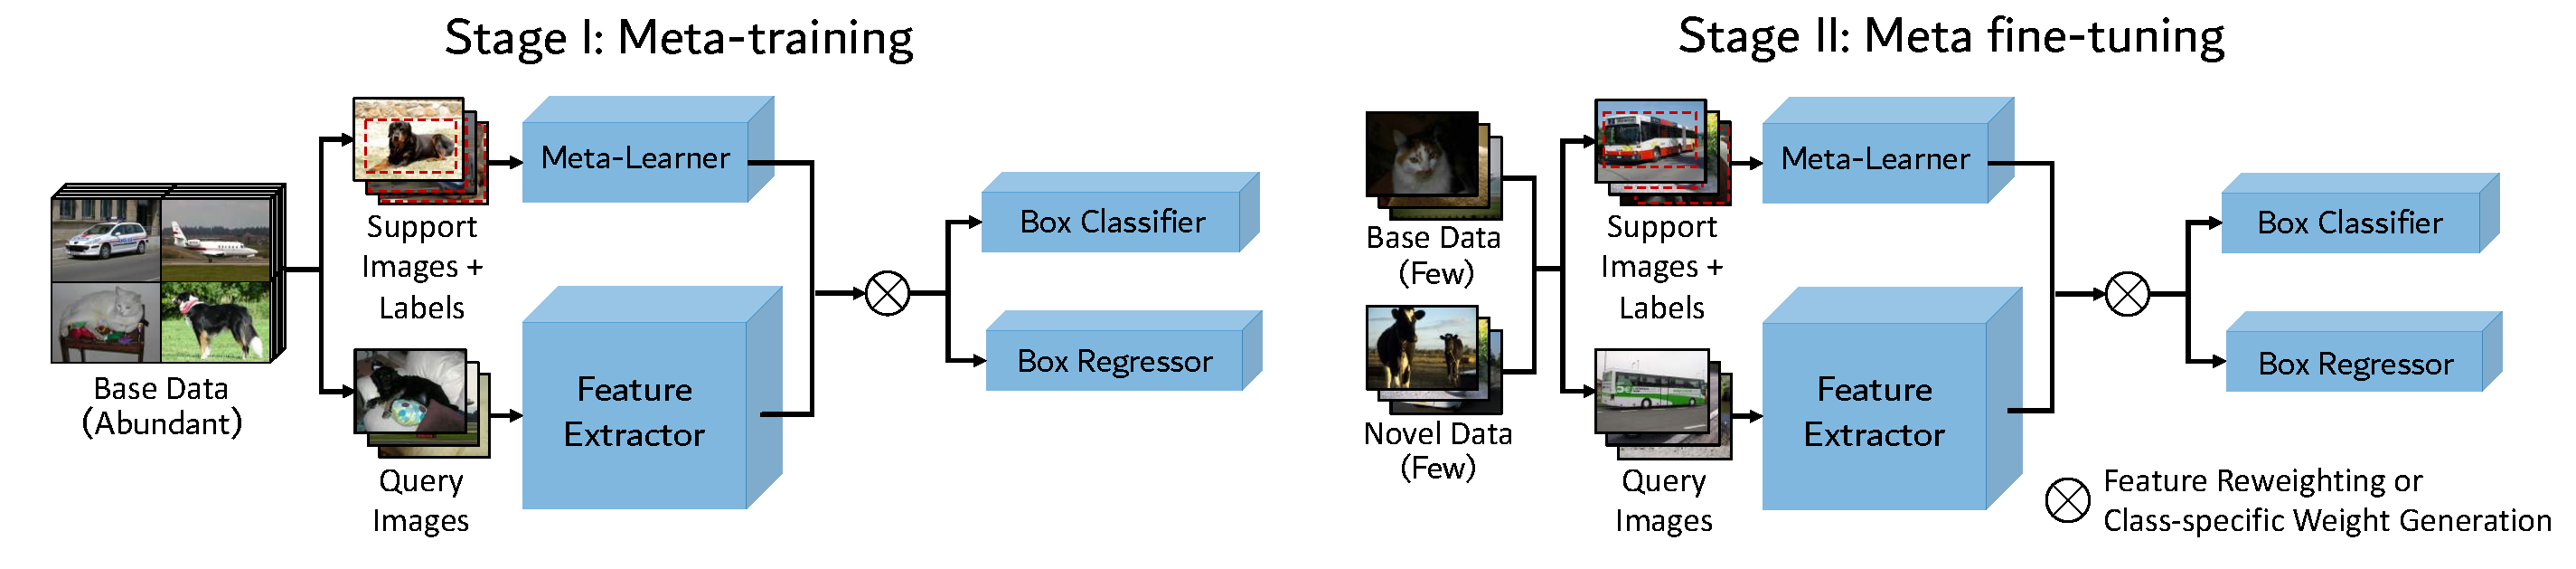
\includegraphics[width=\linewidth]{figs/TFA_fig2.pdf}
    \vspace{-8mm}
    \caption{Abstraction of the meta-learning based few-shot object detectors. A meta-learner is introduced to acquire task-level meta information and help the model generalize to novel classes through feature re-weighting (\textit{e.g.}, FSRW and Meta R-CNN) or weight generation (\textit{e.g.}, MetaDet). A two-stage training approach (meta-training and meta fine-tuning) with episodic learning is commonly adopted.}
    \label{fig:meta_arch}
\end{figure*}

\minisection{Cosine similarity for box classifier.} We consider using a classifier based on cosine similarity in the second fine-tuning stage, inspired by ~\citet{gidaris2018dynamic,qi2018low,chen2019closer}. The weight matrix $W\in\mathbb{R}^{d\times c}$ of the box classifier $\mathcal{C}$ can be written as $[w_1, w_2, ..., w_c]$, where $w_c\in\mathbb{R}^d$ is the per-class weight vector. The output of $\mathcal{C}$ is scaled similarity scores $S$ of the input feature $\mathcal{F}(x)$ and the weight vectors of different classes. The entries in $S$ are 
\begin{equation}
    s_{i,j} = \frac{\alpha \mathcal{F}(x)_i^\top w_j}{\|\mathcal{F}(x)_i\| \|w_j\|}, 
\end{equation}
where $s_{i,j}$ is the similarity score between the $i$-th object proposal of the input $x$ and the weight vector of class $j$. $\alpha$ is the scaling factor. We use a fixed $\alpha$ of 20 in our experiments. We find empirically that the instance-level feature 
normalization used in the cosine similarity based classifier helps reduce the intra-class
variance and improves the detection accuracy of novel classes with less decrease in detection accuracy of base classes when compared to a FC-based classifier, especially when the number of training examples is small.

\subsection{Meta-learning based approaches}
\label{sec:meta}
We describe the existing meta-learning based few-shot object detection networks, including FSRW~\cite{kang2019few}, Meta R-CNN~\cite{yan2019meta} and MetaDet~\cite{wang2019meta}, in 
this section to draw comparisons with our approach.
Figure~\ref{fig:meta_arch} illustrates the structures of these networks.
In meta-learning approaches, in addition to the base object detection model that is either single-stage or 
two-stage, a meta-learner is introduced to acquire class-level meta knowledge and
help the model generalize to novel classes through feature re-weighting, such as FSRW
and Meta R-CNN, or class-specific weight generation, such as MetaDet. The input to the
meta learner is a small set of support images with the bounding box annotations of the target objects. 

The base object detector and the meta-learner are often jointly trained using episodic training~\cite{vinyals2016matching}.
Each episode is composed of a supporting set of $N$ objects and a set of query images.
In FSRW and Meta R-CNN, the support images and the binary masks of the annotated objects are used as input to the meta-learner, which generates class reweighting vectors that modulate the feature representation of the query images.
As shown in Figure~\ref{fig:meta_arch}, the training procedure is also split into a meta-training stage, where the model is only trained on the data of the base classes, and a meta fine-tuning stage, where the support set includes the few examples of the novel classes and a subset of examples from the base classes.

Both the meta-learning approaches and our approach have a two-stage 
training scheme. However, we find that the episodic learning used in meta-learning approaches 
can be very memory inefficient as the number of classes in the supporting set increases. Our
fine-tuning method only fine-tunes the last layers of the network with a normal batch training scheme, which is much more memory efficient. 
